\chapter{الأنواع الكيميائية الطبيعية والاصطناعية}\label{ch:g10:chemical-species}

ملعقة من مثلجات الفانيليا. قد تأتي نكهتها من القرون السوداء لزهرة سحلبية
استوائية، تُقطف وتُعالَج وتُنقع في الكحول أشهرًا؛ وقد تأتي من مصنع يصنع النكهة
من لب الخشب أو من النفط. ذُق الاثنتين جنبًا إلى جنب تجد النكهة الرئيسية
واحدة --- ولسبب وجيه: \omterm{def:g7:atoms-and-molecules:molecule}{فالجزيء} الذي له طعم الفانيليا، الفانيلين، هو \omterm{def:g7:atoms-and-molecules:molecule}{الجزيء}
نفسه تمامًا، أيًّا كانت الطريقة التي حُصل عليه بها. يبيّن هذا الفصل كيف
يستخلص الكيميائيون نوعًا كيميائيًا من نبات، وكيف يصنعونه، وكيف يتحققون من أن
ما حصلوا عليه هو ما يظنونه.

\begin{recall}
\omterm{def:g6:pure-substances-and-mixtures:species}{النوع الكيميائي} صنف معيّن من المواد؛ \omterm{def:g6:pure-substances-and-mixtures:pure-substance}{والمادة النقية} تحوي نوعًا واحدًا ولها
ثوابت محددة، مثل درجتي انصهارها وغليانها
(\cref{ch:g6:pure-substances-and-mixtures}). والسوائل قابلة للامتزاج أو
غير قابلة له، ولكل \omterm{def:g6:solutions-and-solubility:solute}{مذاب} ذوبانيته في كل \omterm{def:g6:solutions-and-solubility:solute}{مذيب}
(\cref{ch:g6:solutions-and-solubility}). \omterm{def:g7:identifying-substances:chromatography}{والكروماتوغرافيا الورقية} تفصل
صبغات \omterm{def:g6:pure-substances-and-mixtures:mixture}{الخليط} (\cref{ch:g7:identifying-substances}).
\end{recall}

\begin{omfigure}
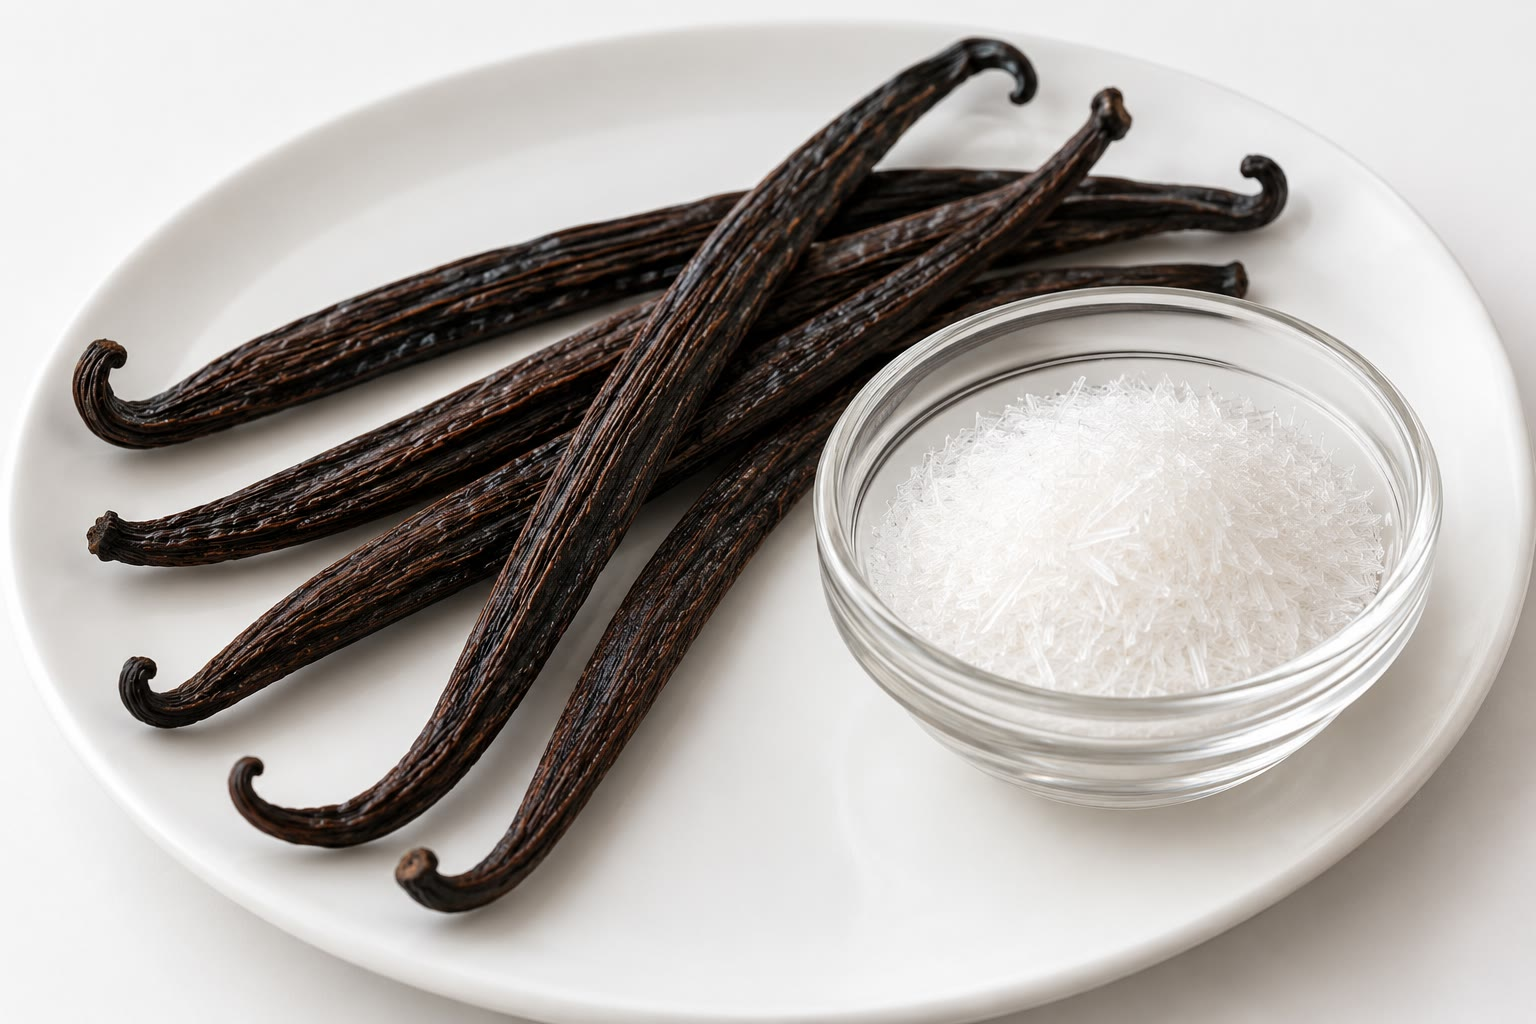
\includegraphics[width=0.55\linewidth]{images/book1/ai/g10-vanilla.jpg}

{\small قرون الفانيليا وبلورات الفانيلين البيضاء: \omterm{def:g7:atoms-and-molecules:molecule}{الجزيء} نفسه، من نبات أو من
مصنع.}
\end{omfigure}

\section{الأنواع الطبيعية والأنواع الاصطناعية}

\begin{definition}[النوع الطبيعي والنوع الاصطناعي]\label{def:g10:chemical-species:natural}
\emph{النوع الطبيعي}\index{نوع طبيعي} \omterm{def:g6:pure-substances-and-mixtures:species}{نوع كيميائي} يصنعه كائن حي أو يوجد
على حاله في الطبيعة. أما \emph{النوع الاصطناعي}\index{نوع اصطناعي} فيصنعه
الكيميائيون من أنواع أخرى بتفاعلات كيميائية. وقد يكون النوع الاصطناعي مطابقًا
لنوع طبيعي (الفانيلين الاصطناعي)، أو لا يكون له نظير في الطبيعة (معظم الأدوية
وأنواع \omterm{def:g8:plastics:plastic}{البلاستيك}).
\end{definition}

\begin{proposition}[النوع نفسه، الخصائص نفسها]\label{prop:g10:chemical-species:same}
\omterm{def:g6:pure-substances-and-mixtures:species}{للنوع الكيميائي} الخصائص نفسها أيًّا كان مصدره: فالفانيلين المصنوع في مصنع
والفانيلين المستخلص من قرن لهما الصيغة نفسها، ودرجة الانصهار نفسها، والرائحة
نفسها. وما قد يختلف هو ما يصحبه: فالمستخلص الطبيعي \omterm{def:g6:pure-substances-and-mixtures:mixture}{خليط}، فيه أنواع أخرى
كثيرة تغيّر طعمه.
\end{proposition}

\begin{history}[من لحاء الصفصاف إلى الأسبرين، 1828--1899]
ظل لحاء الصفصاف قرونًا يُمضغ لمقاومة الحمى والألم. وفي 1828 استخلص منه
كيميائي النوع الفعال، الساليسين؛ ثم حوّله الكيميائيون إلى حمض الساليسيليك،
وهو فعال لكنه يهيّج المعدة. وفي 1897، في شركة للأصباغ والأدوية، صنع فيليكس
هوفمان من حمض الساليسيليك نوعًا اصطناعيًا ألطف: حمض الأسيتيل ساليسيليك،
الذي بيع منذ 1899 باسم الأسبرين. وليس للأسبرين مصدر طبيعي: فهو \omterm{def:g10:chemical-species:natural}{نوع اصطناعي}
خالص.
\end{history}

\section{استخلاص نوع كيميائي}

\begin{definition}[الاستخلاص والاستخلاص سائل--سائل]\label{def:g10:chemical-species:extraction}
\emph{الاستخلاص}\index{استخلاص} إخراج \omterm{def:g6:pure-substances-and-mixtures:species}{نوع كيميائي} من المادة التي تحويه،
عادة بإذابته في \omterm{def:g6:solutions-and-solubility:solute}{مذيب} مختار جيدًا. وفي
\emph{الاستخلاص سائل--سائل}\index{استخلاص سائل--سائل}، يُنقل نوع ذائب في
سائل إلى سائل ثانٍ، \omterm{def:g6:solutions-and-solubility:miscible}{غير قابل للامتزاج} بالأول، \omterm{def:g2:mixing-and-dissolving:dissolve}{يذوب} فيه النوع أفضل؛ ثم يُفصل
السائلان في قمع الفصل.
\end{definition}

\begin{example}[استخلاصات يومية]\label{ex:g10:chemical-species:everyday}
تحضير الشاي \omterm{def:g10:chemical-species:extraction}{استخلاص} بالماء الساخن (النقع الساخن)؛ ونقع قرون الفانيليا في
الكحول \omterm{def:g10:chemical-species:extraction}{استخلاص} بالإيثانول (النقع البارد)؛ وسلق الخضر لتحضير المرق \omterm{def:g10:chemical-species:extraction}{استخلاص}
آخر (الإغلاء).
\end{example}


\begin{definition}[التقطير والتقطير المائي]\label{def:g10:chemical-species:distillation}
\emph{التقطير}\index{تقطير} يسخّن خليطًا سائلًا حتى الغليان، ويعيد البخار
سائلًا في مكثّف يبرّده ماء جارٍ، ويجمع هذا السائل، وهو المقطَّر. أما
\emph{التقطير المائي}\index{تقطير مائي} فيغلي مادة نباتية في الماء: فيحمل
البخار الأنواع العطرية للنبات، التي تنفصل عن الماء في المقطَّر طبقةً زيتية،
هي الزيت العطري.
\end{definition}

\begin{omfigure}
\begin{tikzpicture}[font=\small, scale=0.95]
  \pic[transform shape] at (0,0) {heatingmantle};
  \pic[transform shape] at (0,0) {rbflask={0.55}{omWater!70}};
  \foreach \x/\y in {-0.45/0.35,-0.1/0.55,0.3/0.3,0.5/0.7,-0.6/0.75,0.1/0.9,-0.25/0.2}
    \fill[green!45!black!70] (\x,\y) ellipse (0.09 and 0.04);
  \pic[transform shape] (s) at (0,3.0) {stillhead};
  \pic[transform shape] at ($(s-top)+(0,-0.75)$) {thermometer};
  \pic[transform shape, rotate=-20] (c) at (s-arm) {liebig={3.2}};
  \coordinate (cend) at ($(s-arm)+(-20:3.2)$);
  \pic[transform shape] (a) at (cend) {adapter};
  \pic[transform shape] at ($(a-tip)+(0,-2.3)$) {erlenmeyer={0.18}{omWater!70}};
  \fill[yellow!60!orange!60] ($(a-tip)+(-0.827,-2.3+0.47)$) -- ($(a-tip)+(0.827,-2.3+0.47)$) -- ($(a-tip)+(0.779,-2.3+0.6)$) -- ($(a-tip)+(-0.779,-2.3+0.6)$) -- cycle;
  \draw[<-, omProp, thick] (-0.55,0.55) -- (-2.2,0.9) node[left, text=black, align=right]
    {ماء وأزهار\\ الخزامى};
  \draw[<-, omProp, thick] (1.35,-0.6) -- (2.2,-1.1) node[right, text=black]
    {سترة التسخين};
  \draw[<-, omProp, thick] (0.1,4.2) -- (-1.2,4.6) node[left, text=black] {مقياس الحرارة};
  \draw[<-, omProp, thick] ($(s-arm)+(-20:1.6)+(0,0.32)$) -- ++(0.6,1.0) node[above, text=black]
    {مكثّف يبرّده ماء جارٍ};
  \draw[<-, omProp, thick] ($(a-tip)+(0.4,-1.88)$) -- ++(1.1,0.2) node[right, text=black, align=left]
    {المقطَّر: زيت عطري\\ يطفو على الماء};
\end{tikzpicture}

{\small \omterm{def:g10:chemical-species:distillation}{التقطير المائي} للخزامى. يحمل البخار الزيت العطري إلى المكثّف؛ وينفصل
المقطَّر إلى طبقة رقيقة من الزيت فوق الماء.}
\end{omfigure}

\begin{method}[اختيار مذيب الاستخلاص]\label{met:g10:chemical-species:solvent}
\omterm{def:g10:chemical-species:extraction}{لاستخلاص} نوع من الماء استخلاصًا سائل--سائل يجب أن يكون
\omterm{def:g6:solutions-and-solubility:solute}{المذيب}:
\begin{enumerate}
  \item مذيبًا للنوع أفضل بكثير من الماء؛
  \item \omterm{def:g6:solutions-and-solubility:miscible}{غير قابل للامتزاج} بالماء، حتى تتكوّن طبقتان؛
  \item قليل الخطر قدر الإمكان، وسهل الإزالة بعد ذلك
        (فدرجة غليانه المنخفضة تسمح بتبخيره).
\end{enumerate}
أما أي الطبقتين في الأعلى فتحدده الكثافتان: فالسائل الأقل كثافة
يطفو.
\end{method}

\begin{example}[مذيبات لزيت الخزامى]\label{ex:g10:chemical-species:table}
% ledger: rho:cyclohexane, bp:cyclohexane, rho:ethyl-acetate, bp:ethyl-acetate, rho:CH2Cl2, bp:CH2Cl2, rho:ethanol, bp:ethanol, sol:linalool
اللينالول، النوع الرئيسي في زيت الخزامى، لا \omterm{def:g2:mixing-and-dissolving:dissolve}{يذوب} في الماء إلا بمقدار
\qty{1.6}{g/L}، لكنه \omterm{def:g2:mixing-and-dissolving:dissolve}{يذوب} جيدًا جدًا في المذيبات الآتية:
\begin{center}
\small
\begin{tabular}{lccll}
\hline
\omterm{def:g6:solutions-and-solubility:solute}{المذيب} & كتلة \qty{1}{mL} & يغلي عند & مع الماء & المخاطر الرئيسية \\
\hline
الهكسان الحلقي & \qty{0.78}{g} & \qty{81}{\celsius} & \omterm{def:g6:solutions-and-solubility:miscible}{غير قابل للامتزاج} & قابل للاشتعال، ضار \\
إيثانوات الإيثيل & \qty{0.90}{g} & \qty{77}{\celsius} & \omterm{def:g6:solutions-and-solubility:miscible}{غير قابل للامتزاج} & قابل للاشتعال، مهيّج \\
ثنائي كلورو الميثان & \qty{1.33}{g} & \qty{40}{\celsius} & \omterm{def:g6:solutions-and-solubility:miscible}{غير قابل للامتزاج} & يُشتبه في أنه مسرطن \\
الإيثانول & \qty{0.79}{g} & \qty{78}{\celsius} & \omterm{def:g6:solutions-and-solubility:miscible}{قابل للامتزاج} & قابل للاشتعال \\
\hline
\end{tabular}
\end{center}
لا يمكن استعمال الإيثانول: فهو يمتزج بالماء ولا تتكوّن طبقتان. ومع الهكسان
الحلقي أو إيثانوات الإيثيل تكون طبقة \omterm{def:g6:solutions-and-solubility:solute}{المذيب} في الأعلى؛ ومع ثنائي كلورو
الميثان في الأسفل.
\end{example}

\begin{omfigure}
\begin{tikzpicture}[font=\small, scale=1.2]
  \pic[transform shape] at (0,0) {sepfunnel={omWater!70}{yellow!35!orange!35}};
  \draw[<-, omProp, thick] (0.55,2.1) -- (1.6,2.4) node[right, text=black, align=left]
    {الهكسان الحلقي والزيت\\ (أقل كثافة، في الأعلى)};
  \draw[<-, omProp, thick] (0.55,1.3) -- (1.6,1.2) node[right, text=black, align=left]
    {الماء، يُصرَّف\\ من الصنبور};
  \draw[<-, omProp, thick] (0.25,0.52) -- (1.6,0.4) node[right, text=black] {الصنبور};
\end{tikzpicture}

{\small قمع الفصل بعد الرج والترك: انتقل الزيت إلى الهكسان الحلقي، في
الأعلى.}
\end{omfigure}

\begin{safety}{\ghs[0.8cm]{GHS02}\ghs[0.8cm]{GHS07}\ghs[0.8cm]{GHS08}\ghs[0.8cm]{GHS09}}
% ledger: ghs:cyclohexane
الهكسان الحلقي: شديد القابلية للاشتعال (GHS02)؛ قد يكون قاتلًا إذا ابتُلع ودخل
المسالك التنفسية، ويسبب تهيج الجلد والنعاس (GHS07، GHS08)؛ وشديد السمية
للأحياء المائية (GHS09). يُستعمل تحت ساحبة الغازات، بعيدًا عن
اللهب.
\end{safety}

\section{كروماتوغرافيا الطبقة الرقيقة}

\begin{definition}[كروماتوغرافيا الطبقة الرقيقة]\label{def:g10:chemical-species:tlc}
\emph{كروماتوغرافيا الطبقة الرقيقة}\index{كروماتوغرافيا الطبقة الرقيقة} (TLC)
تفصل الأنواع الكيميائية في \omterm{def:g6:pure-substances-and-mixtures:mixture}{خليط} على صفيحة مغطاة بطبقة رقيقة من مسحوق أبيض
ناعم، هي \emph{الطور الثابت}\index{طور ثابت}. توضع بقع صغيرة من العيّنات على
خط بقلم الرصاص قرب الأسفل؛ وتوقف الصفيحة في حوض مغلق فيه قليل من \omterm{def:g6:solutions-and-solubility:solute}{المذيب}، وهو
\emph{المُزيح}\index{مزيح}، الذي يصعد في الصفيحة ويحمل كل نوع إلى ارتفاع
يتوقف على النوع. ثم تُكشف البقع عديمة اللون بالأشعة فوق البنفسجية أو ببخار
اليود.
\end{definition}

\begin{definition}[معامل الاحتجاز]\label{def:g10:chemical-species:retention-factor}
\emph{معامل الاحتجاز}\index{معامل الاحتجاز} لبقعة هو
\[
  R_f = \frac{\text{المسافة من خط الانطلاق إلى البقعة}}
             {\text{المسافة من خط الانطلاق إلى جبهة المذيب}},
\]
وهو عدد بين 0 و1. ولكل نوع، لصفيحة ومُزيح ودرجة حرارة معيّنة،
$R_f$ خاص به.
\end{definition}

\begin{method}[إجراء كروماتوغرافيا الطبقة الرقيقة وقراءتها]\label{met:g10:chemical-species:tlc}
\begin{enumerate}
  \item ارسم خط الانطلاق بقلم الرصاص على بعد \qty{1}{cm} من الأسفل؛ وضع
        عليه بقعة صغيرة من كل عيّنة ومن كل نوع
        مرجعي.
  \item أوقف الصفيحة في الحوض، \omterm{def:g10:chemical-species:tlc}{والمُزيح} تحت الخط؛ وأغلق
        الحوض.
  \item أخرج الصفيحة حين تصير الجبهة على بعد \qty{1}{cm} تقريبًا من
        الأعلى؛ وعلّم الجبهة فورًا؛ ثم جففها واكشف البقع.
  \item قِس المسافات واحسب $R_f$ لكل بقعة. فالعيّنة التي تعطي بقعة واحدة
        هي على الأرجح نوع نقي؛ والبقعة التي في ارتفاع بقعة مرجعية على
        الصفيحة نفسها هي على الأرجح ذلك
        النوع.
\end{enumerate}
\end{method}

\begin{omfigure}
\begin{tikzpicture}[font=\small, scale=1.25]
  % the tank
  \pic[transform shape] at (0,0) {beaker={0.15}{omWater!80}};
  \fill[white] (-0.55,0.08) rectangle (0.55,1.92);
  \fill[omWater!80] (-0.55,0.08) rectangle (0.55,0.3);
  \draw[omGlass, line width=0.6pt] (-0.55,0.08) rectangle (0.55,1.92);
  \draw[black!60] (-0.55,0.42) -- (0.55,0.42);
  \foreach \x in {-0.3,0,0.3} \fill[black!70] (\x,0.42) circle (0.04);
  \fill[black!25] (-1.0,2.08) rectangle (1.0,2.18);
  \node[anchor=north, align=center] at (0,-0.15) {الحوض، مغلقًا\\ بغطاء};
  % the developed plate
  \begin{scope}[xshift=4.2cm]
    \pic[transform shape] at (0,0) {tlcplate};
    \draw[black!50, dashed] (-0.7,2.8) -- (0.7,2.8);
    \fill[omDef!70] (-0.35,1.36) ellipse (0.1 and 0.07);
    \fill[omDef!70] (-0.35,2.2) ellipse (0.1 and 0.07);
    \fill[omDef!70] (0,1.36) ellipse (0.1 and 0.07);
    \fill[omDef!70] (0.35,2.2) ellipse (0.1 and 0.07);
    \foreach \x/\l in {-0.35/O,0/L,0.35/A} \node[font=\footnotesize, anchor=north] at (\x,0.38) {\l};
    \draw[<->, omProp] (0.95,0.4) -- (0.95,1.36) node[midway, right, text=black, font=\footnotesize] {$d$};
    \draw[<->, omProp] (1.55,0.4) -- (1.55,2.8) node[midway, right, text=black, font=\footnotesize] {$D$};
    \draw[black!40, densely dotted] (-0.25,1.36) -- (0.95,1.36);
    \node[anchor=north, align=center] at (0.2,-0.15) {الصفيحة بعد النشر:\\ $R_f = d/D$};
  \end{scope}
\end{tikzpicture}

{\small \omterm{def:g10:chemical-species:tlc}{كروماتوغرافيا الطبقة الرقيقة} لزيت الخزامى (O) إلى جانب اللينالول (L)
وإيثانوات اللينالين (A). يعطي الزيت بقعتين، في ارتفاعي المرجعين: فهو يحوي
النوعين كليهما. وللينالول، $R_f = d/D$.}
\end{omfigure}

\section{التعرف على نوع كيميائي بثوابته الفيزيائية}

\begin{proposition}[درجة الانصهار تتحقق من الهوية والنقاوة]\label{prop:g10:chemical-species:mp}
% ledger: mp:vanillin, mp:aspirin, mp:salicylic
الجسم الصلب النقي ينصهر انصهارًا حادًا عند درجة حرارة خاصة به: الفانيلين عند
نحو \qty{82}{\celsius}، والأسبرين عند \qty{135}{\celsius}، وحمض الساليسيليك
عند \qty{158}{\celsius}. أما العيّنة غير النقية فتنصهر عند درجة أدنى، وعلى
مدى عدة درجات. ولذلك فقياس درجة الانصهار، على مقعد فلزي مسخّن أو في جهاز
لقياس درجة الانصهار، يتعرف على الجسم الصلب ويبيّن في آن واحد هل هو نقي.
\end{proposition}

\begin{inthelab}[صفيحة كروماتوغرافيا]
يضع التلاميذ بقعًا من زيت الخزامى واللينالول وإيثانوات اللينالين على صفيحة،
وينشرونها في وعاء مغلق \omterm{def:g6:pure-substances-and-mixtures:mixture}{بخليط} من المذيبات يختاره المعلم، ثم يكشفون البقع تحت
مصباح للأشعة فوق البنفسجية، وهم يلبسون نظارات تحجب هذه الأشعة. ويُستعمل
\omterm{def:g10:chemical-species:tlc}{المُزيح} ويُتناول تحت ساحبة الغازات.
\end{inthelab}

\begin{omfigure}
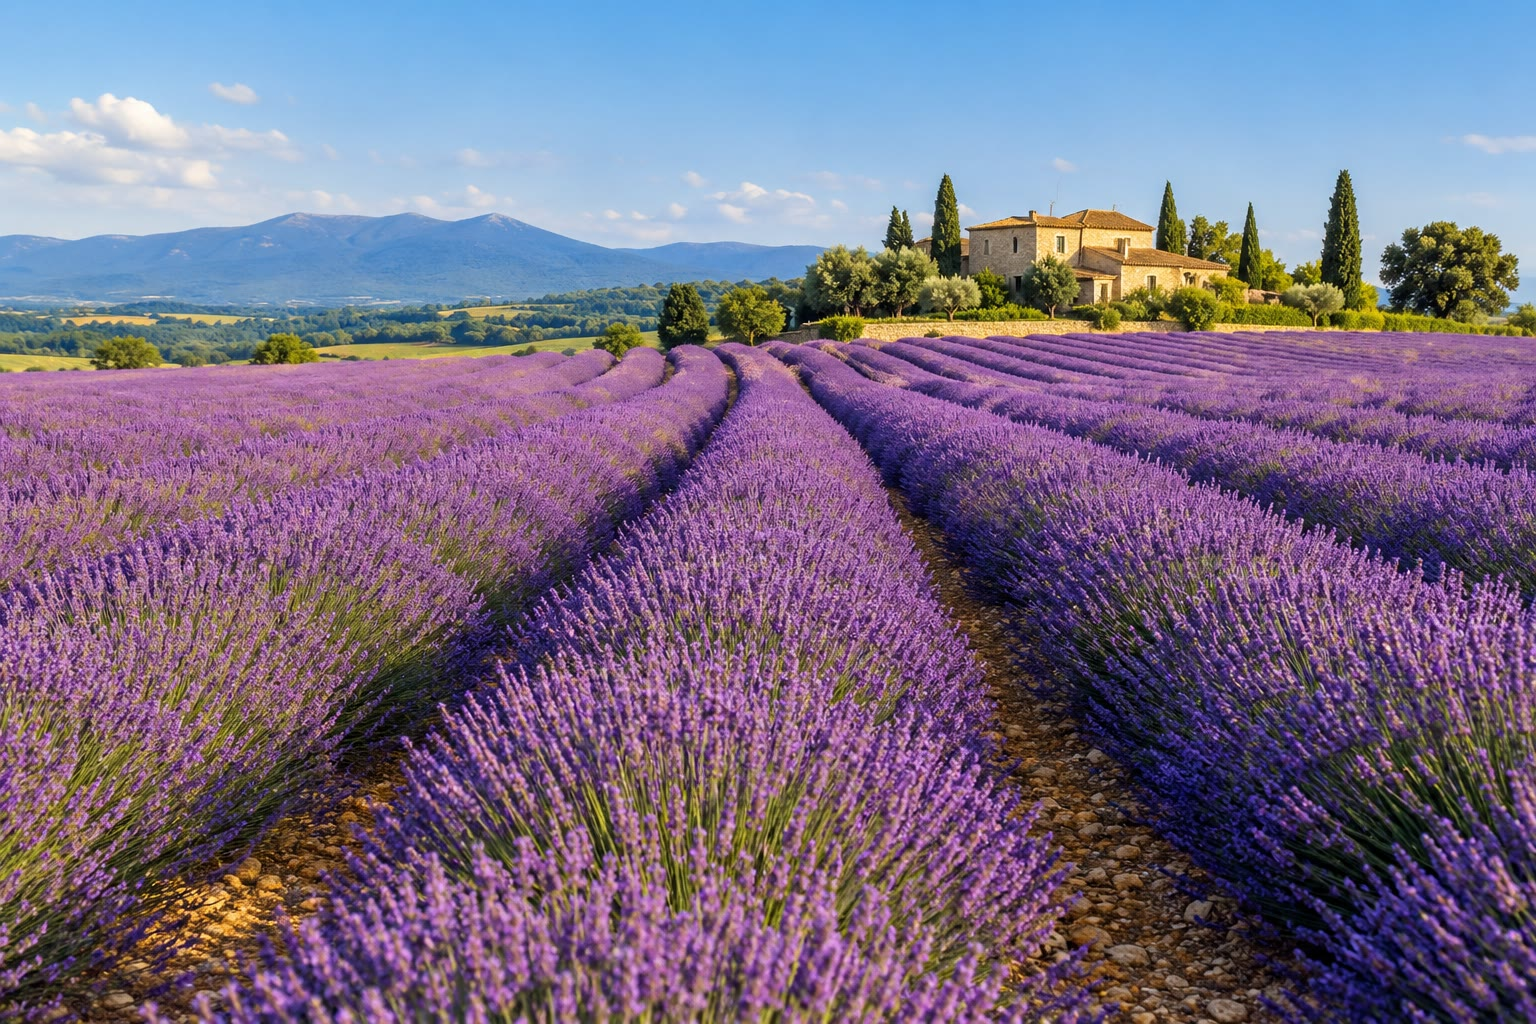
\includegraphics[width=0.55\linewidth]{images/book1/ai/g10-lavender-field.jpg}

{\small حقل خزامى مزهر: \omterm{def:g5:raw-materials-and-recycling:raw-material}{المادة الأولية} لزيت الخزامى
العطري.}
\end{omfigure}

\section{تمارين}

\begin{exercise}[$\star$]\label{exo:g10:chemical-species:1}
\omterm{def:g10:chemical-species:natural}{نوع طبيعي} أم اصطناعي؟ الفانيلين من قرن الفانيليا؛ والأسبرين؛ والكافيين من
حبوب البن؛ والفانيلين المصنوع في مصنع.
\end{exercise}

\begin{exercise}[$\star$]\label{exo:g10:chemical-species:2}
لماذا يكون للفانيلين الاصطناعي والفانيلين الطبيعي درجة الانصهار
نفسها؟
\end{exercise}

\begin{exercise}[$\star$]\label{exo:g10:chemical-species:3}
على صفيحة كروماتوغرافيا، جبهة \omterm{def:g6:solutions-and-solubility:solute}{المذيب} على ارتفاع \qty{6.0}{cm} فوق خط الانطلاق
وبقعة على ارتفاع \qty{2.4}{cm} فوقه. احسب $R_f$ لها.
\end{exercise}

\begin{exercise}[$\star$]\label{exo:g10:chemical-species:4}
اذكر دور المكثّف في \omterm{def:g10:chemical-species:distillation}{التقطير}، وقل لماذا يدخل الماء البارد من طرفه
السفلي.
\end{exercise}

\begin{exercise}[$\star$]\label{exo:g10:chemical-species:5}
اذكر الشروط الثلاثة التي يجب أن يستوفيها \omterm{def:g6:solutions-and-solubility:solute}{مذيب} \omterm{def:g10:chemical-species:extraction}{الاستخلاص}.
\end{exercise}

\begin{exercise}[$\star\star$]\label{exo:g10:chemical-species:6}
مستعينًا بجدول المذيبات، اشرح لماذا لا يمكن استعمال الإيثانول \omterm{def:g10:chemical-species:extraction}{لاستخلاص}
اللينالول من المقطَّر، بينما يمكن استعمال الهكسان الحلقي.
\end{exercise}

\begin{exercise}[$\star\star$]\label{exo:g10:chemical-species:7}
في قمع الفصل يُرج ثنائي كلورو الميثان مع الماء. أي الطبقتين في الأعلى؟ علّل
بالجدول.
\end{exercise}

\begin{exercise}[$\star\star$]\label{exo:g10:chemical-species:8}
مسحوق أبيض يُباع على أنه أسبرين يبدأ في الانصهار عند \qty{126}{\celsius}
وينصهر كليًا عند \qty{132}{\celsius}. ماذا تستنتج؟
\end{exercise}

\begin{exercise}[$\star\star$]\label{exo:g10:chemical-species:9}
انظر إلى شكل الكروماتوغرافيا في هذا الفصل. ماذا يحوي زيت الخزامى؟ وأي
النوعين صعد أعلى؟
\end{exercise}

\begin{exercise}[$\star\star$]\label{exo:g10:chemical-species:10}
رتّب خطوات الحصول على زيت الخزامى في المختبر: فصل الطبقتين؛ \omterm{def:g10:chemical-species:distillation}{والتقطير
المائي}؛ وإضافة الهكسان الحلقي إلى المقطَّر والرج؛ \omterm{def:g3:separating-mixtures:evaporate}{وتبخير} الهكسان
الحلقي.
\end{exercise}

\begin{exercise}[$\star\star$]\label{exo:g10:chemical-species:11}
لماذا يُرسم خط الانطلاق في صفيحة الكروماتوغرافيا بقلم الرصاص ويوضع فوق
\omterm{def:g10:chemical-species:tlc}{المُزيح}؟
\end{exercise}

\begin{exercise}[$\star\star\star$]\label{exo:g10:chemical-species:12}
بعد \omterm{def:g10:chemical-species:extraction}{الاستخلاص} يُزال الهكسان الحلقي بتسخين هادئ، فيبقى الزيت. مستعينًا بدرجتي
غليان الهكسان الحلقي واللينالول (\qty{198}{\celsius})، اشرح
لماذا ينجح ذلك.
\end{exercise}

\begin{exercise}[$\star\star\star$]\label{exo:g10:chemical-species:13}
عيّنة اصطناعية من نكهة تعطي بقعة واحدة على صفيحة كروماتوغرافيا، في ارتفاع
\omterm{def:g10:chemical-species:natural}{النوع الطبيعي}، وتنصهر انصهارًا حادًا عند الدرجة الصحيحة. ما الاستنتاجان
اللذان يمكنك استخلاصهما؟
\end{exercise}

\begin{exercise}[$\star\star\star$]\label{exo:g10:chemical-species:14}
في الكروماتوغرافيا نفسها، للبقعة A $R_f = 0.40$ والجبهة على ارتفاع \qty{5.5}{cm}
فوق الخط. على أي ارتفاع تقع البقعة A؟ ونوع آخر له
$R_f = 0.75$: كم يعلو فوق البقعة A؟
\end{exercise}

\begin{exercise}[$\star\star\star$]\label{exo:g10:chemical-species:15}
يمكن أن \omterm{def:g2:mixing-and-dissolving:dissolve}{يذوب} \qty{1.6}{g} من اللينالول في \qty{1}{L} من الماء. ومقطَّر
من \qty{200}{mL} من الماء يحوي \qty{0.20}{g} من اللينالول الذائب. هل هو
مشبع؟ وكم يستطيع أن يذيب بعدُ؟ ولماذا يستحق هذا الماء أن يُستخلص بالهكسان
الحلقي بدلًا من رميه؟
\end{exercise}

\clearpage % keeps the heading with its problem box (it was stranded at a page foot)
\section{مسألة: عبير الخزامى}

\begin{problem}[{مسألة نهاية الأسبوع --- من سلة من أزهار الخزامى إلى بضع
قطرات من الزيت العطري، يُتحقق منها بالكروماتوغرافيا}]
\label{pb:g10:chemical-species:1}
% ledger: rho:cyclohexane, bp:cyclohexane, rho:CH2Cl2, bp:linalool, ghs:cyclohexane
في مختبر مدرسي تُقطَّر \qty{100}{g} من أزهار الخزامى الطازجة تقطيرًا مائيًا.
فيُرج المقطَّر، وهو عكر، مع \qty{20}{mL} من الهكسان الحلقي في قمع فصل؛
وتُحفظ طبقة الهكسان الحلقي وتُجفف، ثم يُبخَّر الهكسان الحلقي بتسخين هادئ. وما
يبقى هو زيت الخزامى العطري. استعمل جدول المذيبات في هذا
الفصل.

\medskip
\noindent\textbf{الجزء الأول --- \omterm{def:g10:chemical-species:distillation}{التقطير المائي}.}
\begin{enumerate}
  \item ما دور الماء المغلي في \omterm{def:g10:chemical-species:distillation}{التقطير المائي}؟
  \item ما دور المكثّف؟ ومن أين يدخله الماء
        البارد؟
  \item يُظهر المقطَّر طبقة زيتية رقيقة تطفو على الماء. هل الزيت \omterm{def:g6:solutions-and-solubility:miscible}{قابل
        للامتزاج} بالماء؟ وهل هو أكثر كثافة من الماء أم أقل؟
  \item لماذا لا يُكتفى بصب المقطَّر لاسترجاع الزيت؟
\end{enumerate}

\medskip
\noindent\textbf{الجزء الثاني --- \omterm{def:g10:chemical-species:extraction}{الاستخلاص}.}
\begin{enumerate}[resume]
  \item لماذا يُعدّ الهكسان الحلقي مذيبًا مناسبًا لهذا \omterm{def:g10:chemical-species:extraction}{الاستخلاص}؟
  \item هل يمكن استعمال الإيثانول بدلًا منه؟ علّل.
  \item بعد الرج والترك، هل طبقة الهكسان الحلقي في الأعلى أم في
        الأسفل؟ وأين تكون مع ثنائي كلورو الميثان؟
  \item اذكر احتياطين تفرضهما رموز خطر الهكسان الحلقي.
  \item لماذا يمكن \omterm{def:g3:separating-mixtures:evaporate}{تبخير} الهكسان الحلقي دون فقد اللينالول، الذي يغلي
        عند \qty{198}{\celsius}؟
\end{enumerate}

\medskip
\noindent\textbf{الجزء الثالث --- الكروماتوغرافيا.}
توضع بقع من الزيت، ومن اللينالول النقي (L)، ومن إيثانوات اللينالين النقي (A) على
صفيحة كروماتوغرافيا. وبعد النشر تكون الجبهة على ارتفاع \qty{6.0}{cm} فوق خط
الانطلاق. يعطي الزيت بقعتين، عند \qty{2.4}{cm}
و\qty{4.5}{cm}؛ والبقعة L عند \qty{2.4}{cm}، والبقعة A عند \qty{4.5}{cm}.
\begin{enumerate}[resume]
  \item احسب $R_f$ للينالول ولإيثانوات اللينالين.
  \item ماذا يحوي الزيت، بقدر ما تبيّنه هذه الصفيحة؟
  \item هل زيت الخزامى \omterm{def:g6:pure-substances-and-mixtures:pure-substance}{مادة نقية}؟
  \item لماذا وُضعت البقع المرجعية على الصفيحة نفسها التي عليها الزيت؟
  \item يوضع لينالول اصطناعي على صفيحة أخرى نُشرت في الشروط
        نفسها: فلبقعته $R_f = 0.40$. ماذا يمكن أن نستنتج؟
\end{enumerate}

\medskip
\noindent\textbf{الجزء الرابع --- كم من الزيت؟}
يملأ الزيت المحصَّل \qty{1.0}{mL}؛ و\qty{1}{mL} من هذا الزيت يزن
\qty{0.90}{g}.
\begin{enumerate}[resume]
  \item ما كتلة الزيت المحصَّل؟
  \item ما النسبة المئوية لذلك من كتلة الأزهار؟
  \item ما كتلة الأزهار اللازمة للحصول على \qty{100}{g} من الزيت؟
  \item يقال إن الزيت «طبيعي». بأي معنى يصح هذا؟ وهل يختلف لينالوله
        عن اللينالول الاصطناعي؟
  \item اذكر كتلة الزيت العطري المحصَّلة من \qty{100}{g} من
        الأزهار.
\end{enumerate}
\end{problem}
